\documentclass[../main.tex]{subfiles}
\graphicspath{{./images/}}
%%%%%%%%%%%%%%%%%%%%%%%%%%%%%%%%%%%%%%%%%%%%%%%%%%%%%%%%%%%%%%%%%

\begin{document}
Some concepts introduced in this thesis are important but not necessarily core elements in the detection and recognition of objects in dense environments. They are derived to this section, the appendix, where they are properly explained and put in context with the rest of the work without cluttering the main body of the report.

\section{Seam Carving} \label{sec:seam_carving}
Section \ref{sec:2D_approach} states the issue of having proper tooling to create quality datasets. Apart from labeling tools, already mentioned in the section, there are image processing-related tools that can be of use. In particular tools that can change the size of the image without distorting the important information inside. This is quite useful since most computer vision models, old or new, require homogeneous image sizes. Standard image resizing (like the one in Microsoft Word or any other text processing tool) is based in interpolating the pixels in the image. This, however, distorts the overall look of the contents in the image. If the resizing is too big, objects may look too thinly stretched or too wide. This, of course, may affect the algorithms' performance. An alternative to resizing is cropping, but that may not be always possible if the objects of interest are close to the sides of the image. 

In an attempt to alleviate this and provide with a strong method to resize images to collect homogeneous datasets in size, this thesis introduces an implementation of the \emph{seam carving} algorithm. The seam carving algorithm was introduced in \cite{seamcarving} and improved in \cite{seamcarving_improved} as a ``content-aware image resizing" algorithm. Fundamentally, the seam carving algorithm computes an energy map of the input image and reduces lines of pixels incrementally, always attempting to follow the path of minimum energy, and hence affecting the original image as little as possible. The seam carving algorithm as developed in \cite{seamcarving_improved} has been implemented in Python with the aid of Numba\footnote{To accelerate loops over the pixels, which would otherwise take many minutes if the input image is high resolution.}, and embedded into the labeling Graphical User Interface introduced in Section \ref{sec:2D_approach}. Its mathematical theory is explained below.

\paragraph{Seam carving with backward energy}
Here the original algorithm from \cite{seamcarving} is detailed, and from it the \emph{forward energy} improvement from \cite{seamcarving_improved} is later explained. The authors do not specifically name it ``backward'', but that is the standard naming of the algorithm in contrast to the ``forward'' version, which is the actual name given by the authors.

The first step is to compute a measure of the energy in the image. To do so, the Sobel operator is applied to obtain the edges in the image. The algorithm should avoid areas with high magnitude, and hence containing lots of edges, and cut through those that are uniform. Doing so, a map the same size as the input image is obtained with a measure of energy per pixel. The aim is now to find what set of adjacent pixels from bottom to top can be removed by distorting as little as possible the overall energy. In other words: what seam of pixels can I remove the path of which has the minimum energy. This is not trivial to compute. The path in a 2D image from bottom to top can not be computed by brute force, that would take too much to compute\footnote{$O(2^{\text{height*width}})$ to be precise.}. And a greedy approach wouldn't provide optimal results. The authors approach this problem with dynamic programming: having the energy map, they compute a new map containing the \emph{accumulated energy} from bottom top. Every pixel in this new map contains the minimal energy that would be needed to go from its position to the top, and is constructed row by row. The first row in the accumulated energy map is the same as the one in the energy map obtained by computing the Sobel operator. The second row is the sum of the corresponding column in the energy map plus the lowest-valued adjacent pixel, meaning by adjacent the pixel above, diagonal right or diagonal left. Row by row the accumulated energy map is computed. Looking at its last row, the index of lowest-valued element is the minimum energy required to go back to the top (to go back to the first row). The path's shape can be obtained by simply tracing back the lowest energy pixels. This is exemplified in figure \ref{fig:dynprog_example}.

Once a seam is found, the pixels belonging to that seam are eliminated. If the user requested to reduce the size further, then the algorithm is repeated. This algorithm is not only useful to reduce the width of images, it can also be used to reduce their height if the image is rotated 90 degrees.

\paragraph{Seam carving with forward energy}
The seam carving algorithm is by no means perfect. See for instance \ref{fig:seam_carved_bench}, where the bench's feet are too slender and the horizontal wooden back is otherwise untouched. Quoting \cite{seamcarving_improved}, seam carving with the backward energy algorithm ``is focused on removing seams with the least amount of energy, ignoring energy that is introduced into the images and video by applying the operator''. To counter this, they introduce a new criterion that no longer ignores the energy that is inserted into the resized image after removing the seam. Now, the inserted energy due to the new edges created after the seam removal are computed into the accumulated energy map, as depicted in figure \ref{fig:forward_energy_diagram}. Options (a), (b) and (c) account for possible vertical seam costs for pixel $p_{i,j}$ when the red pixels are removed, and new edges are created. The three possible vertical seam costs (removing the one on the diagonal left, the one up and the one on the diagonal right, wrt $p_{i,j}$) are stored in matrices, like so

\begin{equation}
    \begin{array}{l}
    \text{(a)} \; C_{L}(i, j)=|I(i, j+1)-I(i, j-1)|+|I(i-1, j)-I(i, j-1)| \\
    \text{(b)} \; C_{U}(i, j)=|I(i, j+1)-I(i, j-1)| \\
    \text{(c)} \; C_{R}(i, j)=|I(i, j+1)-I(i, j-1)|+|I(i-1, j)-I(i, j+1)|
    \end{array}
\end{equation}
Where $I(i, j)$ is the value from 0 to 255 of the grayscale input image in pixel $(i, j)$. This allows to store in matrices $C_{L}$, $C_{U}$ and $C_{R}$ the cost of the new frontier created by removing $p_{i-1, j-1}$, $p_{i-1, j}$ and $p_{i-1, j+1}$ respectively. The accumulated energy matrix $M$ is then computed as
\begin{equation}
    M(i, j)=P(i, j)+\min \left\{\begin{array}{l}
    M(i-1, j-1)+C_{L}(i, j) \\
    M(i-1, j)+C_{U}(i, j), \\
    M(i-1, j+1)+C_{R}(i, j)
    \end{array}\right.
\end{equation}
Where $P(i, j)$ is an additional weighting measure\footnote{Also known as \emph{mask}.} that can be introduced by the user, in case some areas are user-defined as high cost areas that should not be removed (like the pixels inside a face). For the current implementation it has been left to 0 for all $i$ and $j$.

To compare results of the backward and forward algorithms see figures \ref{fig:seam_carved_testbench_front}, \ref{fig:seam_carved_castle}, \ref{fig:seam_carved_bench}.
 

\begin{figure}[htbp]
    \centering
    \resizebox{0.8\linewidth}{!}{\import{images/}{dynprog_example.pgf}}
    \caption{An example of the dynamic programming approach to find the minimum energy path from bottom to top (shown in red font). The matrix on the left is an energy map ranging from 0 to 1, similar to the one that could be obtained from applying the Sobel filter to an image. From it the accumulated energy from the bottom to the top is computed (matrix on the right, referred to as $M$). The minimum energy path will begin at its lowest valued column of the first row, and move down from there by picking the lowest valued adjacent pixel. As the path is being constructed its indices are stored, and once the full path is found the overall image's horizontal size is reduced by one column, precisely eliminating those pixels from the path.}
    \label{fig:dynprog_example}
\end{figure}

\begin{figure}[htbp]
    \centering
    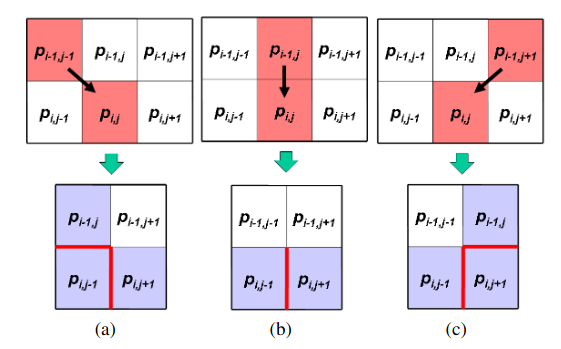
\includegraphics[width=0.6\linewidth]{images/forward_energy_diagram.png}
    \caption{The three possible seam costs for pixel $p_{i,j}$ with forward energy. Light blue represents the new pixel neighbors after removing the seam, and the red lines the new frontiers. Image extracted from \cite{seamcarving_improved}.}
    \label{fig:forward_energy_diagram}
\end{figure}

\begin{figure}[htbp]
    \centering
    \resizebox{1\linewidth}{!}{\import{images/}{seam_carved_testbench_front.pgf}}
    \caption{Comparison of the backward and forward energy methods for an actual image of the testbench. The image on the left is the energy map, where the brightest points mean more energy. The areas of highest density look like inverted triangles, unsurprisingly, since they represent the cost of going from bottom of the image to the top. In other words, seams starting from the base of a Coca-Cola or Pepsi can will have a high accumulated energy all throughout the can's area. As it can be guessed by the axis, the input image has been reduced by 550 pixels horizontally and 300 pixels vertically. Oddly enough, the best result comes from using the backward energy method. This is generally not the case.}
    \label{fig:seam_carved_testbench_front}
\end{figure}

\begin{figure}[htbp]
    \centering
    \resizebox{1\linewidth}{!}{\import{images/}{seam_carved_castle.pgf}}
    \caption{Same as in figure \ref{fig:seam_carved_testbench_front}. This image perfectly represents the usefulness of the seam carving method: it maintains the aspect ratio of both the person and the castle by deleting seams in the middle. The image is ``easy'' enough to provide good results with the forward and backward energy methods. Image from Wikimedia Commons.}
    \label{fig:seam_carved_castle}
\end{figure}

\begin{figure}[htbp]
    \centering
    \resizebox{1\linewidth}{!}{\import{images/}{seam_carved_bench.pgf}}
    \caption{This bench image is a good example on the improvement that the forward energy algorithm carries: it preserves the integrity of the feet by taking into account the energy coming from the neighbors of the potential seam.}
    \label{fig:seam_carved_bench}
\end{figure}


\section{Random Sample Consensus (RANSAC)} \label{sec:ransac}
The Random Sample Consensus \cite{ransac_paper81} technique is a widely used method to estimate model parameters in data with inliers and outliers. It is based in a voting scheme, where random subsets of points vote for different model parameters and only the best one is kept. The details of the algorithm are presented in \ref{lst:ransac_algo}, but in essence does the following: from the set of points (or data values) in the dataset, a random subset is chosen. The minimum number of points for said subset will depend on the model that the user wants (a line will require at least 2, a plane 3, and so on). With this subset, the model parameters are estimated (using a Least Squares method for instance), and then the remainder of the set of points is introduced. From these new introduced points, those at a distance closer than a threshold $t$ are considered inliers, and the rest are considered outliers. A measure of how well the points fit the estimated model parameters is computed, also called the error, and stored. The process is repeated again a number of iterations (defined by the user too) only keeping the best model parameters, that is, those having a lower error than the previous iteration.

\begin{algorithm}[h]
    \SetAlgoLined
    Set t, max\_iterations, d\\
    iterations = 0\\
    best\_fit = None\\
    best\_error = $\infty$\\
    \While{iterations $<$ max\_iterations}{
        // select a random subset of points\\
        inliers := select\_inliers\_random()\\
        model\_params := fit\_inliers\_to\_model(inliers)\\
        also\_inliers := \{ \} // empty set\\
        // see what of the remaining points in the data set are inliers\\
        \For(){points in data that not in inliers}{
            \If{Error(model\_params, point) $<$ t}{
                add point to also\_inliers
            }
        }
        \If{length(also\_inliers) $>$ d}{
            // unite inliers sets
            inliers = inliers + also\_inliers\\
            // test how good the model is and get a fitting error\\
            better\_model := fit(inliers)\\
            current\_error := Error(better\_model, inliers)\\
            \If{current\_error $<$ best\_error}{
                best\_fit := better\_model\\
                best\_error := current\_error\\
            }
        }
        iterations := iterations + 1\\
    }
    return best\_fit\\
    \caption{The standard Random Sample Consensus (RANSAC) algorithm}
    \label{lst:ransac_algo}
\end{algorithm}

How to choose a number of iterations? What is the likelihood of finding the correct number of parameters? To answer these questions one requires the outlier ratio (at least an approximation) $e$, defined as the ratio between the number of outliers divided by the total number of points in the set; and the number of minimum sampled points $s$ required to fit the model (again, 2 for a line, 3 for a plane and so on). The number of iterations will be called $T$ and the probability of taking all $s$ inliers is called $p$.  

With this being said, what is the probability drawing an inlier from the set of points? $1-e$. And the probability of drawing $s$ inliers? $\left(1-e\right)^{s}$. Hence, the probability of failing in one iteration is $1-\left(1-e\right)^{s}$ (that is, taking at least one point that is not an inlier). This leaves the equation below:

\begin{equation}
    1-p=\left(1-(1-e)^{s}\right)^{T}
\end{equation}

Taking the natural logarithm at both sides of the equation, and isolating T, results in

\begin{equation} \label{eq:ransac_T}
    T=\frac{\log (1-p)}{\log \left(1-(1-e)^{s}\right)}
\end{equation}

With equation \ref{eq:ransac_T} one can determine the number of iterations $T$ for a desired probability $p$. For example, for a probability of 99\% of finding the $s=3$ inliers and an outlier ratio of $e=0.8$ the number of trials $T=574$.

\end{document}